\documentclass[aspectratio=169, 11pt]{beamer}

\usetheme{Madrid}
\usecolortheme{seahorse}
\setbeamertemplate{navigation symbols}{}
\setbeamertemplate{footline}[frame number]
\setbeamertemplate{itemize items}[circle]
\setbeamerfont{frametitle}{size=\large, series=\bfseries}

\usepackage{booktabs}
\usepackage{graphicx}
\usepackage{amsmath}
\usepackage{hyperref}
\usepackage{tikz}

\title{COVID-19 Diagnosis Prediction Under Noisy Labels}
\subtitle{Fixing the Data Before Fixing the Model}
\author{Cyrus Chung \and Hussain Elahi \and Kayin Malcolm \and Sohail (Neel) Sarkar}
\institute{STA314, University of Toronto}
\date{March 2026}

\begin{document}

% ============================================================
% SLIDE 1: Title
% ============================================================
\begin{frame}
\titlepage
\begin{center}
  \vspace{-1.2em}
  {\normalsize Team \textbf{Unemployed\_Statisticians} \quad $\mid$ \quad Final Rank: \textbf{\#2} \quad $\mid$ \quad Private Score: \textbf{0.99130}}
\end{center}
\end{frame}

% ============================================================
% SLIDE 2: The Task and the Twist
% ============================================================
\begin{frame}{The Task and the Twist}
\textbf{Binary classification:} predict whether a patient tested positive for COVID-19 from symptoms, demographics, and clinical indicators.

\vspace{0.4em}
\begin{columns}[T]
\begin{column}{0.48\textwidth}
  \textbf{Dataset at a glance}
  \begin{itemize}
    \item $\sim$1{,}500 training rows, $\sim$3{,}500 test rows
    \item 18 features: 3 continuous, 2 categorical, 13 binary
    \item Balanced classes (778 pos.\ / 722 neg.)
    \item \texttt{comorbidity} 53\% NaN, recoded as ``None''
  \end{itemize}
\end{column}
\begin{column}{0.48\textwidth}
  \textbf{The catch}
  \begin{itemize}
    \item The instructor \textit{deliberately flipped} a subset of training labels
    \item Roughly \textbf{19\% of labels are wrong}
    \item Models trained on noisy labels plateaued at 74\% to 80\%
    \item Scored on \textbf{accuracy}: you get the label right or you do not
  \end{itemize}
\end{column}
\end{columns}

\vspace{0.4em}
\centering
\textit{Label noise shaped our entire approach.}
\end{frame}

% ============================================================
% SLIDE 3: Data Overview and Feature Importance
% ============================================================
\begin{frame}{Data Overview and Feature Importance}
\begin{columns}[T]
\begin{column}{0.40\textwidth}
  {\small
  \begin{itemize}
    \item \texttt{oxygen\_level} dominates (importance $\approx$ 18)
    \item \texttt{age} and \texttt{body\_temperature} are next
    \item Key symptoms: \texttt{dry\_cough}, \texttt{shortness\_of\_breath}, \texttt{loss\_of\_smell}
    \item Many binary features contribute $<$ 5\% each but collectively matter
  \end{itemize}
  }
\end{column}
\begin{column}{0.57\textwidth}
  \centering
  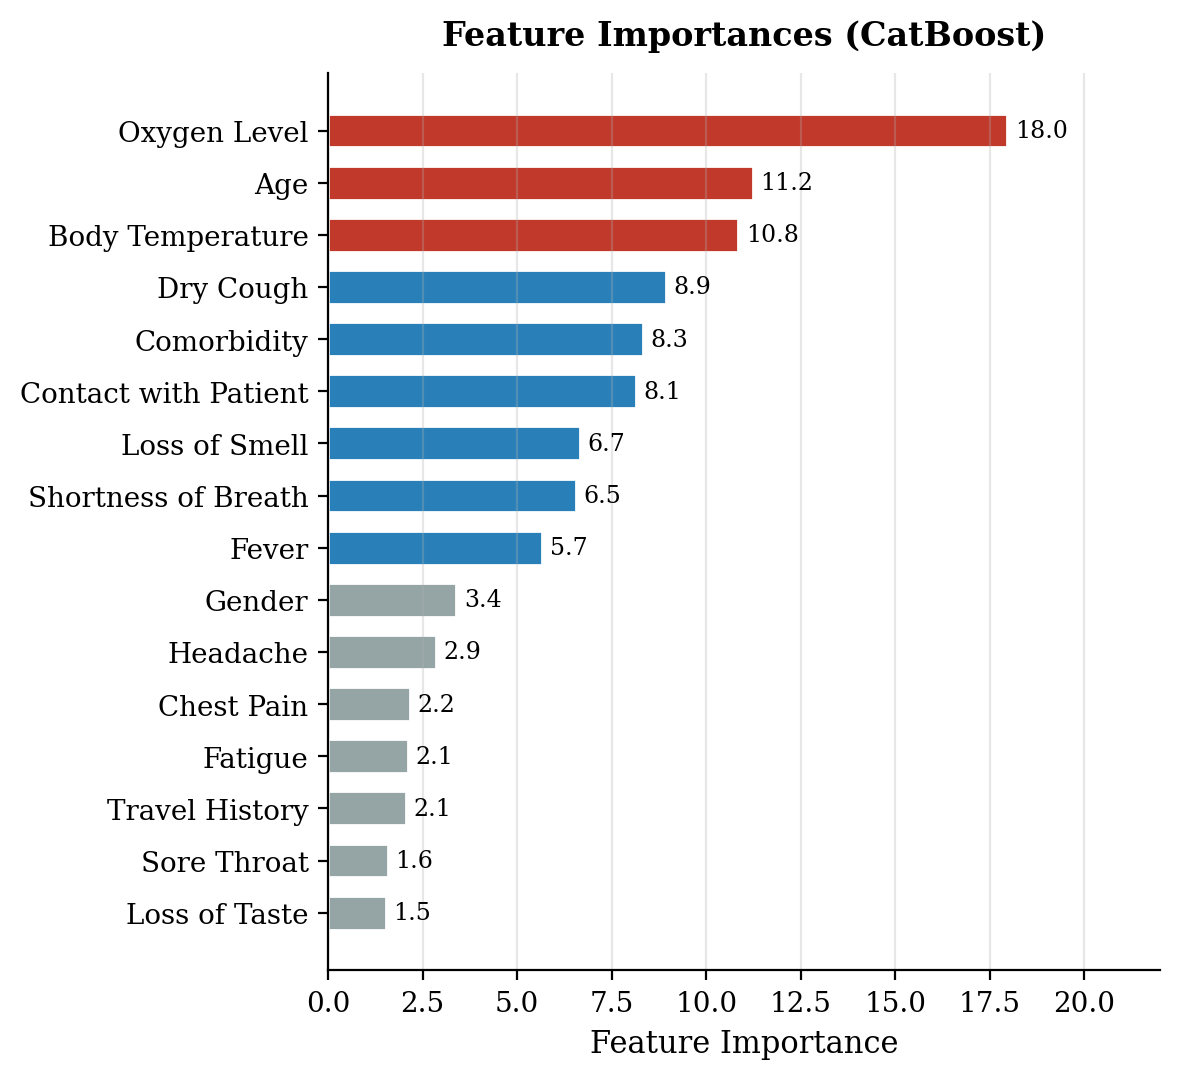
\includegraphics[width=0.92\textwidth, height=0.70\textheight, keepaspectratio]{figures/fig_features.png}
  \vspace{0.1em}

  {\footnotesize CatBoost feature importances (exploratory).}
\end{column}
\end{columns}
\end{frame}

% ============================================================
% SLIDE 4: Why Standard Models Fail Here
% ============================================================
\begin{frame}{Why Standard Models Fail Here}

\textbf{The core issue:} with $\sim$19\% label noise, any model that fits training labels hard will learn the noise.\n\n{\small
\begin{center}
  \begin{tabular}{lcc}
    \toprule
    \textbf{Model} & \textbf{CV Accuracy} & \textbf{Problem} \\
    \midrule
    CatBoost (Optuna-tuned)     & 0.7487 & Memorises noisy labels \\
    LightGBM                    & 0.7673 & Same issue \\
    LDA                         & 0.7567 & Linear, underpowered \\
    QDA                         & 0.7167 & High variance, small $n$ \\
    GaussianNB                  & 0.7013 & Assumes feature independence \\
    $k$-NN ($k$=31)             & 0.7047 & Noise in neighbours \\
    \midrule
    Logistic Regression (T1+T2) & 0.9147 & Decent after label correction \\
    \textbf{TabPFN 5-seed (T1+T2)}  & \textbf{0.9460} & \textbf{Best by far} \\
    \bottomrule
  \end{tabular}
\end{center}
}

\begin{itemize}
  \item All tree-based and classical models hit 0.70 to 0.77 on \textit{noisy} labels. No tuning broke through.
  \item Even LR jumps to 0.91 once labels are fixed. The bottleneck was \textbf{label quality}, not model complexity.
\end{itemize}
\end{frame}

% ============================================================
% SLIDE 5: What TabPFN Is and Why It Fits This Problem
% ============================================================
\begin{frame}{What is TabPFN?}

\textbf{TabPFN} (Hollmann et al., 2022) is a transformer \textit{meta-trained} on millions of synthetic tabular classification datasets.

\vspace{0.3em}
\begin{columns}[T]
\begin{column}{0.55\textwidth}
  \textbf{How it works}
  \begin{itemize}
    \item The entire training set is fed as \textit{context} in a single forward pass, similar to prompting an LLM
    \item Predictions via \textbf{in-context learning}: no gradient updates, no fine-tuning on your data
    \item Approximates the Bayesian posterior predictive:\\$P(y_{\text{test}} \mid X_{\text{test}},\, X_{\text{train}},\, y_{\text{train}})$
  \end{itemize}
\end{column}
\begin{column}{0.42\textwidth}
  \textbf{Why it fits our task}
  \begin{enumerate}
    \item \textbf{Pre-training = regularisation.} Cannot overfit to 1{,}500 rows since it never trains on them via gradient descent
    \item \textbf{Noise robustness.} Bayesian posterior smooths over individual flipped labels
    \item \textbf{No hyperparameters.} Zero risk of overfitting to CV folds
  \end{enumerate}
\end{column}
\end{columns}

\vspace{0.3em}
Binary classification is the natural sweet spot for TabPFN. The prior was meta-trained heavily on 2-class tasks, and the output space (a single probability) is simple and well-calibrated.
\end{frame}

% ============================================================
% SLIDE 6: Noise Detection, Three Methods
% ============================================================
\begin{frame}{Noise Detection: Three Independent Methods}

Instead of relying on any single noise detection technique, we ran three methods that use \textit{completely different} signals and combined their outputs.

\vspace{0.5em}
\textbf{Method 1: Confident Learning (Cleanlab).}\\
5-fold OOF logistic regression $\to$ Cleanlab estimates joint distribution of noisy vs.\ true labels.\\
Flagged \textbf{285} samples (19.0\%).

\vspace{0.4em}
\textbf{Method 2: Area Under the Margin (AUM, CatBoost).}\\
Compute margin $m_i(t) = P_t(\text{true class}) - P_t(\text{other class})$ at 5 CatBoost checkpoints (100 to 500 iters).\\
Samples with mean AUM $< 0.40$ are consistently hard-to-learn. Flagged \textbf{352} samples.

\vspace{0.4em}
\textbf{Method 3: Dataset Cartography.}\\
5 seeds $\times$ 5 folds of LR $\to$ mean per-sample confidence $P(\text{true label})$.\\
Hard-to-learn threshold: mean confidence $< 0.45$. Flagged \textbf{302} samples.

\vspace{0.4em}
\textit{One method is probabilistic, one is margin-based, one is training-dynamics-based.\\What matters is where they agree.}
\end{frame}

% ============================================================
% SLIDE 7: Consensus Tiers and Label Correction
% ============================================================
\begin{frame}{Consensus Tiers and Label Correction}
\begin{columns}[T]
\begin{column}{0.45\textwidth}
  \textbf{Voting rule:} count how many of 3 methods flagged each sample.

  \vspace{0.3em}
  \begin{itemize}
    \item \textbf{Tier 1} (all 3 agree): \textbf{215} samples\\
          $\to$ Label flipped. Near-certain noise.
    \item \textbf{Tier 2} (2 of 3 agree): \textbf{81} samples\\
          $\to$ Label flipped. Probable noise.
    \item \textbf{Tier 3} (0 or 1 method): \textbf{1{,}204} samples\\
          $\to$ Label retained as given.
  \end{itemize}

  \vspace{0.3em}
  \textbf{Total corrected: 296 labels.}

  \vspace{0.2em}
  {\small This is a precision/recall tradeoff on noise detection itself. We chose precision: flipping a correct label is just as damaging as keeping a wrong one.}
\end{column}
\begin{column}{0.52\textwidth}
  \centering
  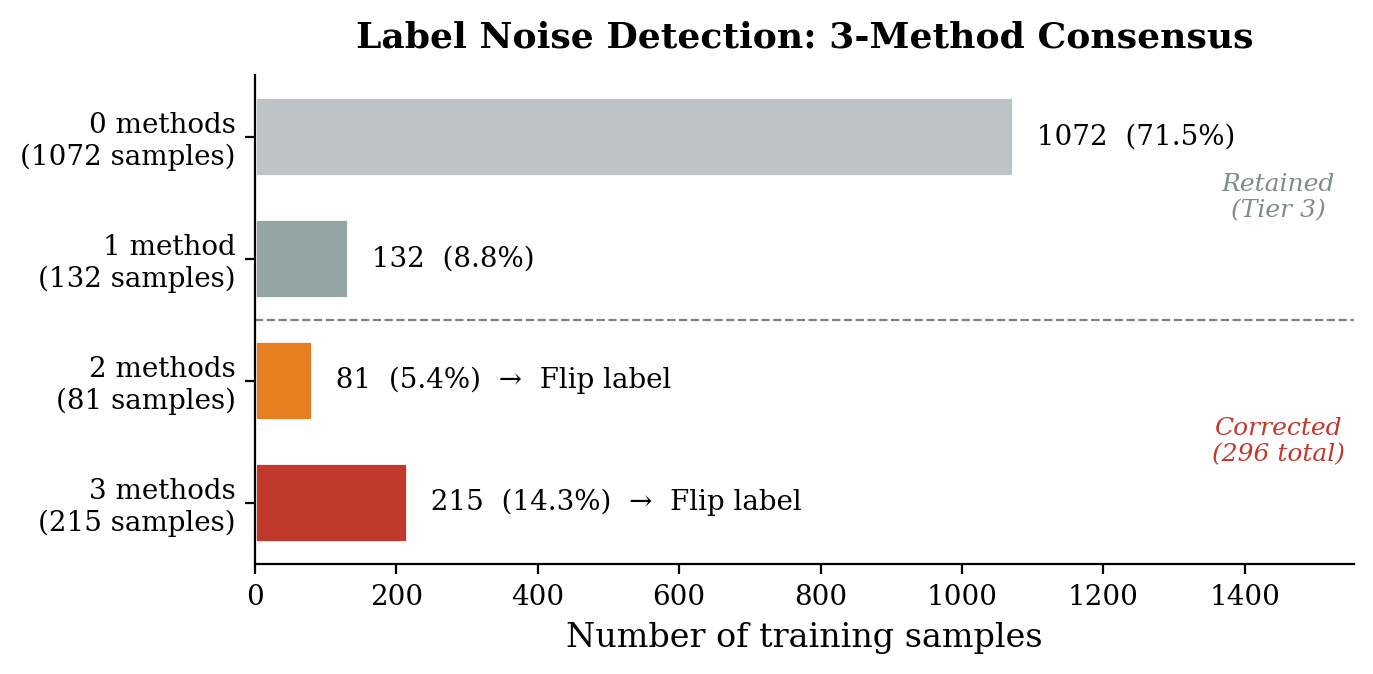
\includegraphics[width=\textwidth]{figures/fig_tiers.png}
\end{column}
\end{columns}
\end{frame}

% ============================================================
% SLIDE 8: Impact of Label Correction
% ============================================================
\begin{frame}{Impact: Before vs.\ After Label Correction}
\begin{columns}[T]
\begin{column}{0.48\textwidth}
  \centering
  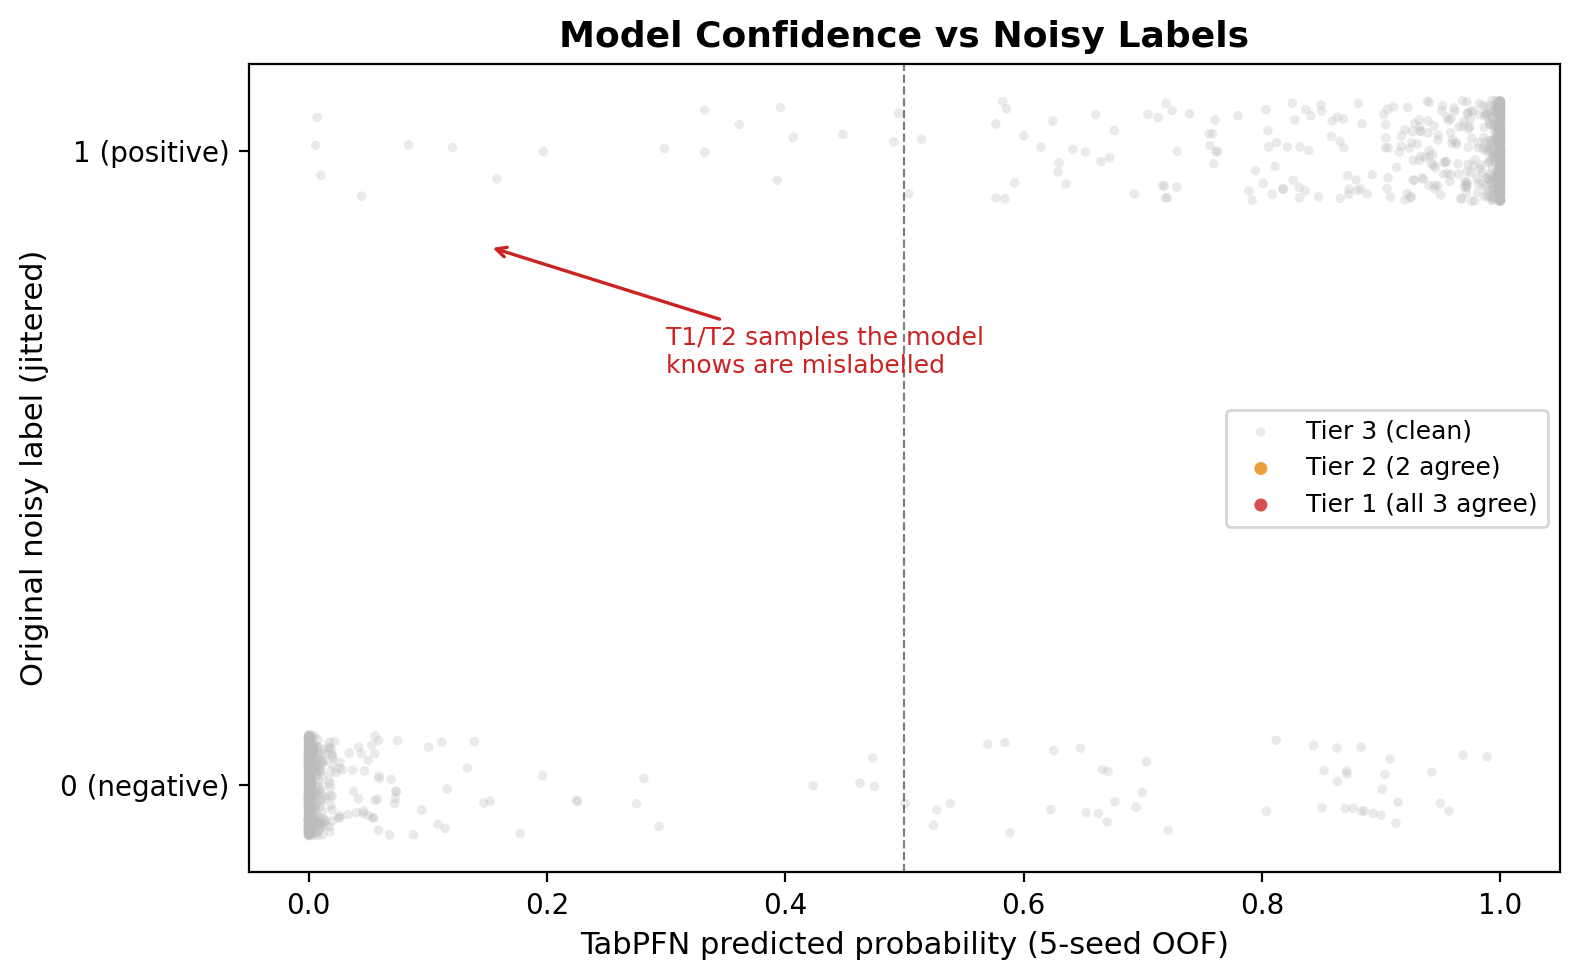
\includegraphics[width=0.90\textwidth]{figures/confidence_vs_labels.png}

  \vspace{0.2em}
  {\small TabPFN OOF probabilities vs.\ original labels.\\
  Clusters in the lower-right and upper-left\\ are the corrected samples.}
\end{column}
\begin{column}{0.48\textwidth}
  \textbf{Progression of private scores:}

  \vspace{0.2em}
  {\small
  \begin{tabular}{lc}
    \toprule
    \textbf{Strategy} & \textbf{Private} \\
    \midrule
    S1: T1 only      & 0.99015 \\
    S2: +Features     & 0.98261 $\downarrow$ \\
    S3: T1+T2         & 0.99073 \\
    \textbf{S4: 5-seed}   & \textbf{0.99130} \\
    \bottomrule
  \end{tabular}
  }

  \vspace{0.3em}
  \begin{itemize}
    \item S1$\to$S3: Tier 2 corrections give \textbf{+0.00058}
    \item S2: feature engineering \textit{hurt} ($-0.00754$)
    \item S3$\to$S4: 5-seed ensemble adds \textbf{+0.00057}
    \item 10 total submissions, no leaderboard probing
  \end{itemize}
\end{column}
\end{columns}
\end{frame}

% ============================================================
% SLIDE 9: The 5-Seed Ensemble
% ============================================================
\begin{frame}{The 5-Seed Ensemble: Variance Reduction}

\textbf{Problem:} TabPFN has stochastic internal processing. Different random seeds produce slightly different probability estimates.

\vspace{0.3em}
\textbf{Solution:} Train with 5 seeds (42, 123, 314, 777, 2026), average the probability vectors.

\vspace{0.3em}
\begin{columns}[T]
\begin{column}{0.50\textwidth}
  \textbf{Pipeline per seed:}
  \begin{enumerate}
    \item 5-fold stratified CV $\to$ OOF probabilities
    \item Full-train model $\to$ test probabilities
    \item Repeat for all 5 seeds
  \end{enumerate}
  $\Rightarrow$ 25 OOF estimates per training sample\\
  $\Rightarrow$ 5 test prediction vectors, averaged
\end{column}
\begin{column}{0.47\textwidth}
  \textbf{Why this works:}
  \begin{itemize}
    \item This is \textit{not} diversity-based ensembling (blending different model types)
    \item It is pure \textbf{variance reduction} over the same architecture
    \item Blending TabPFN with LR actually \textit{hurt} (0.9220 vs.\ 0.9460). Diluting a strong model with a weaker one reduces signal.
  \end{itemize}
\end{column}
\end{columns}

\vspace{0.5em}
\centering
Final prediction: classify at threshold 0.50. Threshold sweeping on OOF showed no meaningful gain.
\end{frame}

% ============================================================
% SLIDE 10: Kaggle Progression
% ============================================================
\begin{frame}{Competition Trajectory}
\begin{columns}[T]
\begin{column}{0.55\textwidth}
  \centering
  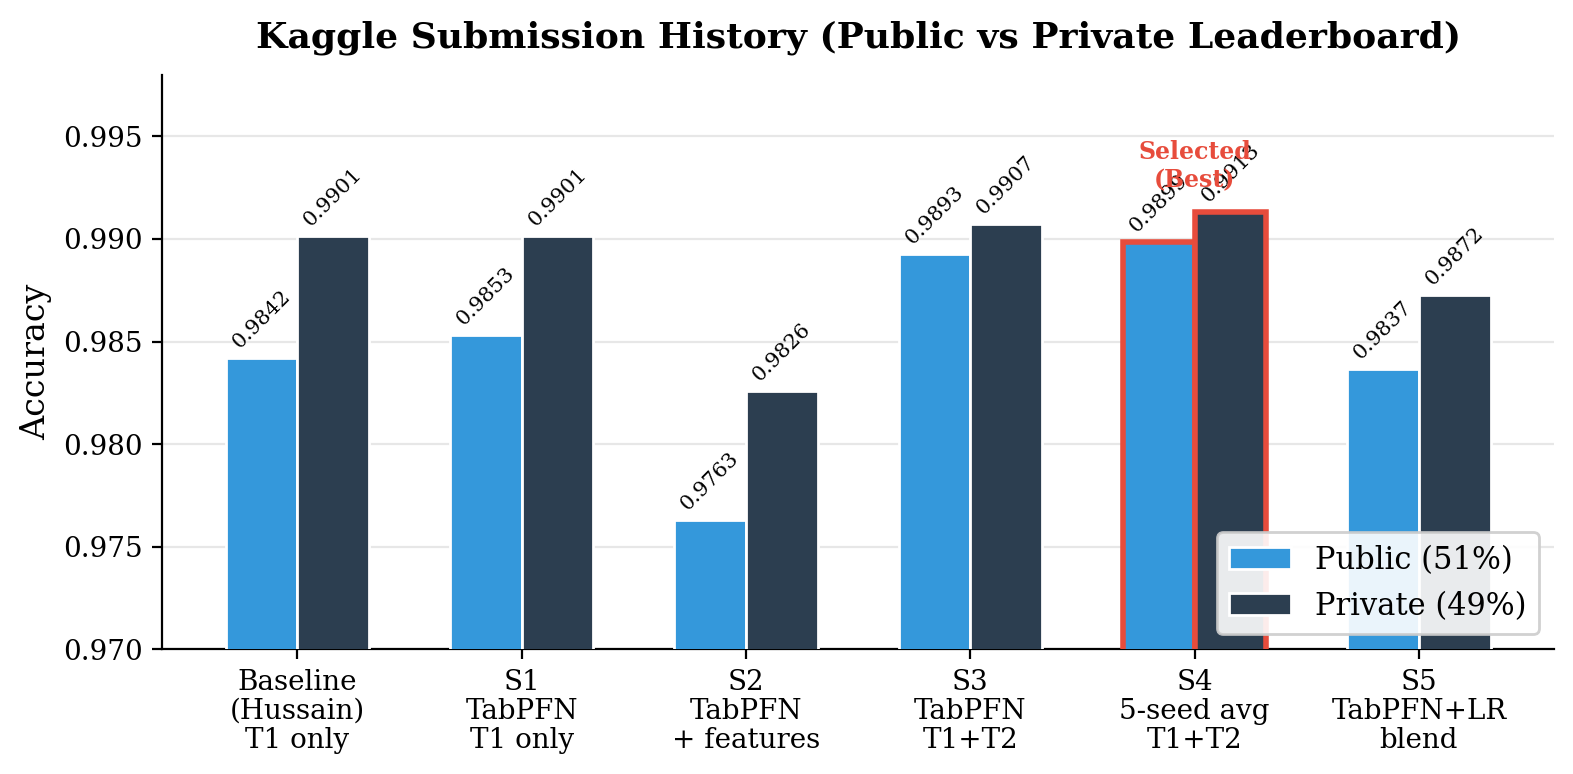
\includegraphics[width=\textwidth]{figures/fig_kaggle.png}
\end{column}
\begin{column}{0.42\textwidth}
  \begin{itemize}
    \item Only \textbf{10 total submissions}; deliberate, not leaderboard-probing
    \item Each submission tested exactly one hypothesis
    \item Private (0.99130) $>$ Public (0.98985)\\
          $\to$ \textbf{no overfitting to public split}
    \item S2 (feature eng.) was the only regression, confirming TabPFN's prior $>$ hand-crafted features
    \item Final rank: \textbf{\#2 overall}
  \end{itemize}
\end{column}
\end{columns}
\end{frame}

% ============================================================
% SLIDE 11: Key Takeaways
% ============================================================
\begin{frame}{Key Takeaways}

\begin{enumerate}
  \item \textbf{Label quality matters more than model complexity.}\\
        Every model trained on noisy labels hit a ceiling of 74\% to 80\%. After cleaning 296 labels, we hit 99\%+.

  \vspace{0.3em}
  \item \textbf{Consensus-based noise detection is safer than any single method.}\\
        Three independent signals agreeing on the same sample is strong evidence. Voting filters false positives.

  \vspace{0.3em}
  \item \textbf{Pre-trained transformers \textit{can} work on tabular data, under the right conditions.}\\
        Small $n$, binary classification, clean(ed) labels. In-context learning avoids overfitting.

  \vspace{0.3em}
  \item \textbf{Feature engineering can hurt when the model's prior is already stronger.}\\
        On 1{,}500 rows, TabPFN's inductive bias outperformed manual interactions.

  \vspace{0.3em}
  \item \textbf{Ensemble the same strong model; do not blend with weaker ones.}\\
        Multi-seed averaging reduces variance. Blending with LR diluted the signal.
\end{enumerate}
\end{frame}

% ============================================================
% SLIDE 12: Conclusion
% ============================================================
\begin{frame}{Conclusion}

\begin{center}
  {\Large\bfseries Private Score: 0.99130 \quad$\boldsymbol{\mid}$\quad Rank: \#2}
\end{center}

\vspace{0.5em}
\begin{columns}[T]
\begin{column}{0.48\textwidth}
  \textbf{What we did}
  \begin{itemize}
    \item 3-method noise detection pipeline
    \item 296 label corrections (215 T1 + 81 T2)
    \item TabPFN v2, 5-seed ensemble
    \item No feature engineering, no threshold tuning
    \item 10 principled submissions
  \end{itemize}
\end{column}
\begin{column}{0.48\textwidth}
  \textbf{What mattered most}
  \begin{itemize}
    \item The jump from $\sim$0.75 CV accuracy to 0.99 on Kaggle came from \textbf{fixing labels}
    \item Clean data did the heavy lifting, not model choice
    \item Private $>$ Public confirms no overfitting
  \end{itemize}

  \vspace{0.4em}
  \textbf{Future work}
  \begin{itemize}
    \item Pseudo-labelling of confident test predictions
    \item Extending correction into Tier 3
  \end{itemize}
\end{column}
\end{columns}

\vspace{0.8em}
\centering
{\small Code: \url{https://github.com/n33levo/unemployed_statistician}}
\end{frame}

\end{document}
